\documentclass[a4paper,11pt]{article}
\input{/home/tof/Documents/Cozy/latex-include/preambule_doc.tex}
\input{/home/tof/Documents/Cozy/latex-include/preambule_commun.tex}
\newcommand{\showprof}{show them}  % comment this line if you don't want to see todo environment
\setlength{\fboxrule}{0.8pt}
\fancyhead[L]{\fbox{\Large{\textbf{Archi 12}}}}
\fancyhead[C]{\textbf{Exercices RIP}}
\newdate{madate}{10}{09}{2020}
%\fancyhead[R]{\displaydate{madate}} %\today
\fancyhead[R]{Terminale - NSI}
\fancyfoot[L]{\vspace{1mm}Christophe Viroulaud}
\AtEndDocument{\label{lastpage}}
\fancyfoot[C]{\textbf{Page \thepage/\pageref{lastpage}}}
\fancyfoot[R]{\includegraphics[width=2cm,align=t]{/home/tof/Documents/Cozy/latex-include/cc.png}}

\begin{document}
\begin{exo}
    \begin{center}
        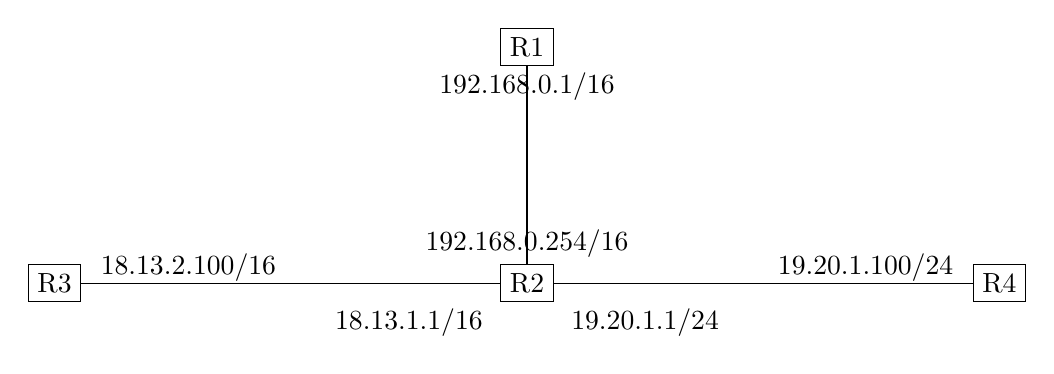
\begin{tikzpicture}
            \node[draw] (A) at (0,3) {R1};
            \node[draw] (B) at (0,0) {R2};
            \node[draw] (C) at (-6,0) {R3};
            \node[draw] (D) at (6,0) {R4};
            \node[yshift=-0.5cm] at (A) {192.168.0.1/16};
            \node[yshift=0.5cm] at (B) {192.168.0.254/16};
            \node[xshift=1.5cm,yshift=-0.5cm] at (B) {19.20.1.1/24};
            \node[xshift=-1.5cm,yshift=-0.5cm] at (B) {18.13.1.1/16};
            \node[xshift=1.7cm,yshift=0.2cm] at (C) {18.13.2.100/16};
            \node[xshift=-1.7cm,yshift=0.2cm] at (D) {19.20.1.100/24};
            \draw (A) -- (B);
            \draw (C) -- (B);
            \draw (B) -- (D);
        \end{tikzpicture}
        \captionof{figure}{Réseau étudié}
        \label{reseau}
    \end{center}
    On a exécuté le protocole RIP sur le réseau figure \ref{reseau}.
    \begin{enumerate}
        \item Donner l'adresse des trois réseaux.
        \item Donner la table de routage du routeur R1.
    \end{enumerate}
\end{exo}
\begin{exo}\textbf{Extrait du sujet 0 du bac blanc 2021: }
On considère un réseau composé de plusieurs routeurs reliés de la façon suivante :
\begin{center}
\centering
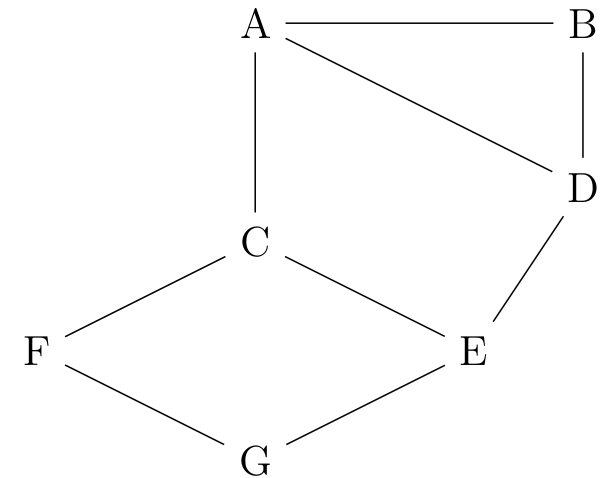
\includegraphics[width=6cm]{ressources/exo-bac.png}
\label{IMG}
\end{center}
\begin{center}
\centering
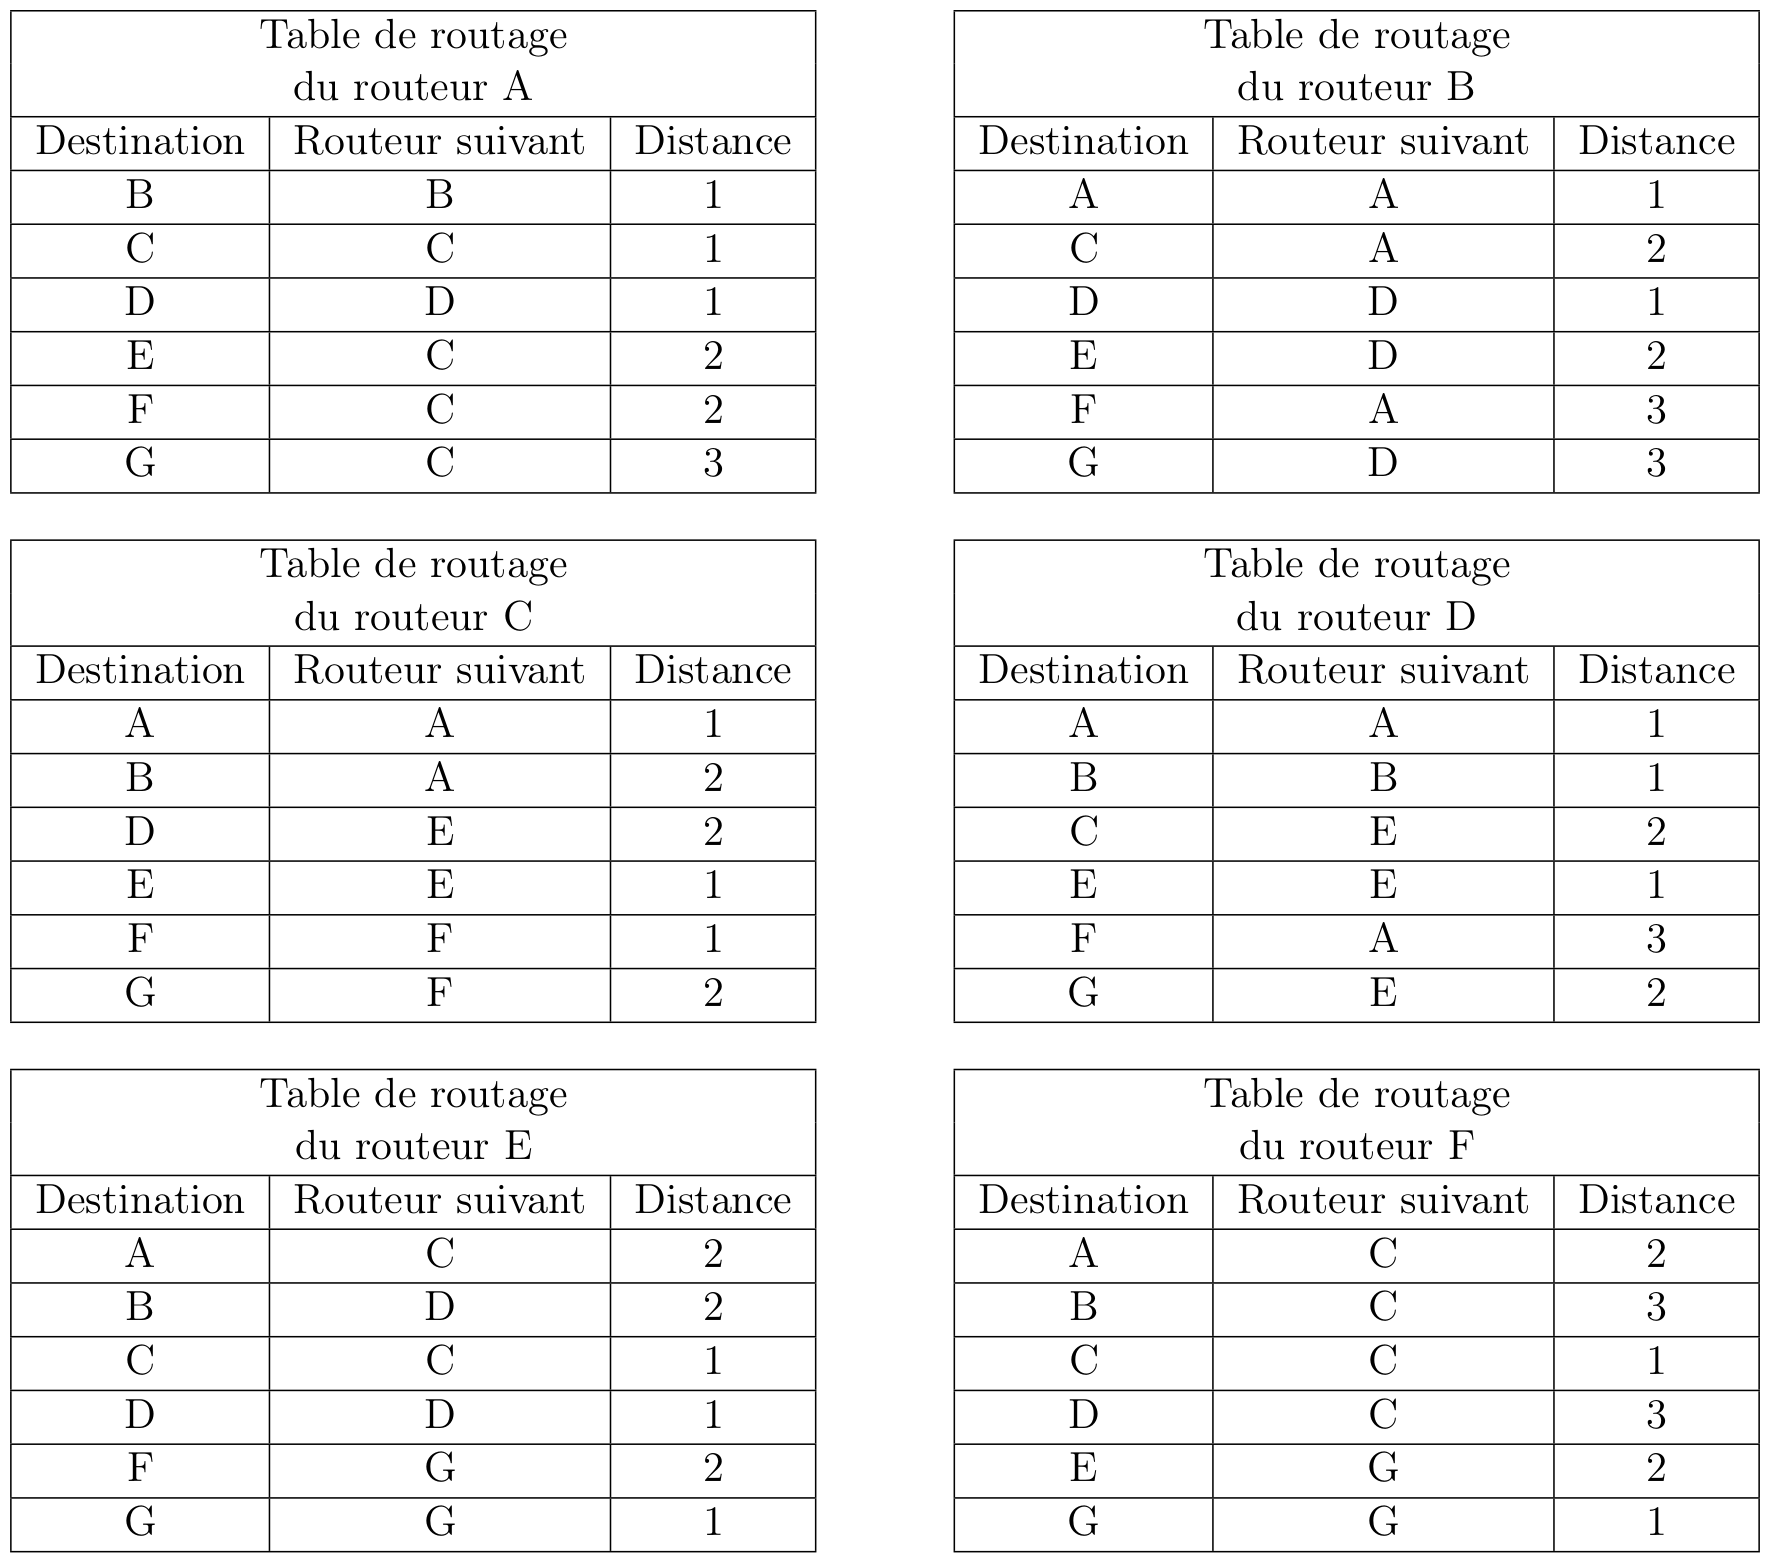
\includegraphics[width=12cm]{ressources/exo-bac-tables.png}
\captionof{figure}{Tables de routage}
\label{IMG}
\end{center}
\begin{enumerate}
    \item Le routeur A doit transmettre un message au routeur G, en effectuant un nombre minimal de sauts. Déterminer le trajet parcouru.
    \item Déterminer une table de routage possible pour le routeur G obtenu à l’aide du protocole RIP.
\end{enumerate}
\end{exo}
\begin{exo}
    \begin{center}
        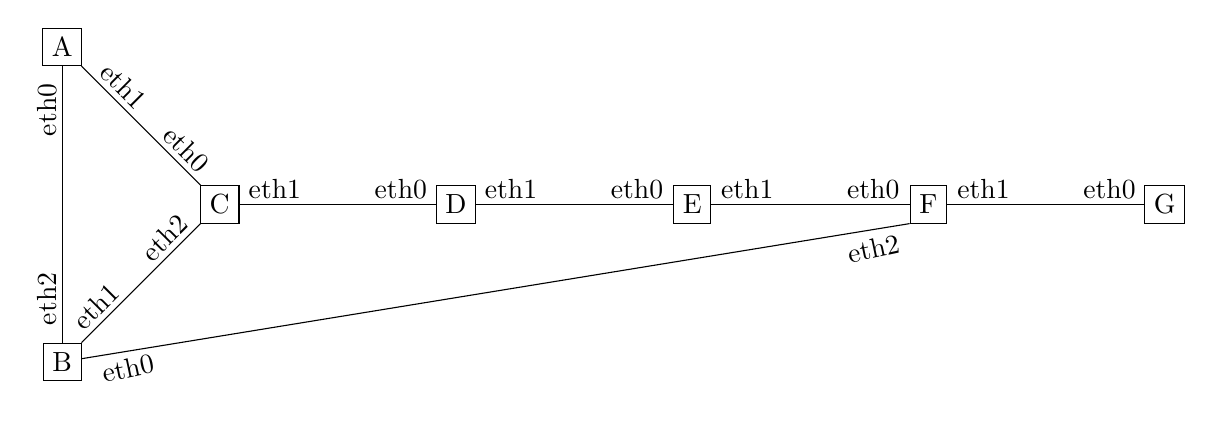
\begin{tikzpicture}
            \node[draw] (A) at (-2,2) {A};
            \node[draw] (B) at (-2,-2) {B};
            \node[draw] (C) at (0,0) {C};
            \node[draw] (D) at (3,0) {D};
            \node[draw] (E) at (6,0) {E};
            \node[draw] (F) at (9,0) {F};
            \node[draw] (G) at (12,0) {G};
            \node[rotate=90,xshift=-0.8cm,yshift=0.2cm] at (A) {eth0};
            \node[rotate=90,xshift=0.8cm,yshift=0.2cm] at (B) {eth2};
            \node[rotate=-45,xshift=0.9cm,yshift=0.2cm] at (A) {eth1};
            \node[rotate=-45,xshift=-0.8cm,yshift=0.2cm] at (C) {eth0};
            \node[rotate=45,xshift=0.8cm,yshift=0.2cm] at (B) {eth1};
            \node[rotate=45,xshift=-0.8cm,yshift=0.2cm] at (C) {eth2};
            \node[xshift=0.7cm,yshift=0.2cm] at (C) {eth1};
            \node[xshift=-0.7cm,yshift=0.2cm] at (D) {eth0};
            \node[xshift=0.7cm,yshift=0.2cm] at (D) {eth1};
            \node[xshift=-0.7cm,yshift=0.2cm] at (E) {eth0};
            \node[xshift=0.7cm,yshift=0.2cm] at (E) {eth1};
            \node[xshift=-0.7cm,yshift=0.2cm] at (F) {eth0};
            \node[xshift=0.7cm,yshift=0.2cm] at (F) {eth1};
            \node[xshift=-0.7cm,yshift=0.2cm] at (G) {eth0};
            \node[rotate=12,xshift=-0.8cm,yshift=-0.4cm] at (F) {eth2};
            \node[rotate=12,xshift=0.8cm,yshift=-0.25cm] at (B) {eth0};

            \draw (A) -- (B);
            \draw (A) -- (C);
            \draw (C) -- (B);
            \draw (C) -- (D);
            \draw (D) -- (E);
            \draw (E) -- (F);
            \draw (F) -- (G);
            \draw (F.south west) -- (B);
        \end{tikzpicture}
        \captionof{figure}{Réseau étudié}
        \label{reseau2}
    \end{center}
    On a exécuté le protocole RIP sur le réseau figure \ref{reseau2}.
    \begin{enumerate}
        \item Donner la table de routage de A après la phase d'initialisation.
        \item Après une période d'échanges les tables sont stabilisées. Donner, pour chaque routeur, l'extrait de table pour la destination G.
        \item On suppose que la connexion B-F tombe en panne. Quel vecteur de distance est envoyé par B à ses voisins pour atteindre G?
        \item Pour chacun des événements ci-après donner le cas du cours qui est appliqué par le routeur, en réponse à la demande RIP:
              \begin{itemize}
                  \item Les routeurs A et C reçoivent de B l'information (le vecteur) de la question précédente.
                  \item Le routeur C retransmet ce même vecteur à D.
                  \item Le routeur D transmet le vecteur (G, 3) à C.
              \end{itemize}
        \item Après le dernier cas ci-avant quel vecteur est transmis par C à A?
    \end{enumerate}
\end{exo}
\end{document}